\item \textbf{For each dataset, examine the stationarity of the residuals using the ACF and PACF functions, Lag Plots, and/or other approaches. Show your results and provide commentary about your observations.}

\textit{\gls{ADF} shows that the time series is non-stationary or stationary. If the p-value is less than the significance level of 0.05 and the \gls{ADF} statistic is lower than one of the critical values, then the time series is stationary. For example, tables \ref{tab:Ass1_D1_ADF} and \ref{tab:Ass1_D2_ADF} shows the result of \gls{ADF} on a residual component of STL method in the two datasets.}

\begin{table}[H]
\centering
\caption{The result of the \gls{ADF} on the first dataset.}
\label{tab:Ass1_D1_ADF}
\begin{tabular}{lr}
\toprule
{} &            0 \\
\midrule
ADF Statistic               &   -24.697687 \\
p-value                     &     0.000000 \\
\#Lags Used                  &     3.000000 \\
Number of Observations Used &  3646.000000 \\
Critical Value (1\%)         &    -3.432145 \\
Critical Value (5\%)         &    -2.862333 \\
Critical Value (10\%)        &    -2.567192 \\
\bottomrule
\end{tabular}

\end{table}

\begin{table}[H]
\centering
\caption{The result of the \gls{ADF} on the second dataset.}
\label{tab:Ass1_D2_ADF}
\begin{tabular}{lr}
\toprule
{} &             0 \\
\midrule
ADF Statistic               & -1.128610e+01 \\
p-value                     &  1.416821e-20 \\
\#Lags Used                  &  2.700000e+01 \\
Number of Observations Used &  2.792000e+03 \\
Critical Value (1\%)         & -3.432694e+00 \\
Critical Value (5\%)         & -2.862576e+00 \\
Critical Value (10\%)        & -2.567321e+00 \\
\bottomrule
\end{tabular}

\end{table}



\textit{\gls{KPSS} is another test for checking the stationarity of a time series. If the p-value is less than the significance level of 0.05, then the time series is not stationary. Table \ref{tab:Ass1_D1_KPSS} and \ref{tab:Ass1_D2_KPSS} show the result of this test on STL residual.}

\begin{table}[H]
\centering
\caption{The result of the \gls{KPSS} on the first dataset.}
\label{tab:Ass1_D1_KPSS}
\begin{tabular}{lr}
\toprule
{} &          0 \\
\midrule
KPSS Statistic        &   0.318117 \\
p-value               &   0.100000 \\
Lags Used             &  22.000000 \\
Critical Value (10\%)  &   0.347000 \\
Critical Value (5\%)   &   0.463000 \\
Critical Value (2.5\%) &   0.574000 \\
Critical Value (1\%)   &   0.739000 \\
\bottomrule
\end{tabular}

\end{table}

\begin{table}[H]
\centering
\caption{The result of the \gls{KPSS} on the second dataset.}
\label{tab:Ass1_D2_KPSS}
\begin{tabular}{lr}
\toprule
{} &          0 \\
\midrule
KPSS Statistic        &   0.017052 \\
p-value               &   0.100000 \\
Lags Used             &  68.000000 \\
Critical Value (10\%)  &   0.347000 \\
Critical Value (5\%)   &   0.463000 \\
Critical Value (2.5\%) &   0.574000 \\
Critical Value (1\%)   &   0.739000 \\
\bottomrule
\end{tabular}

\end{table}

\textit{We can conclude that the series is stationary or not based on both \gls{KPSS} and \gls{ADF} \cite{StationarityStatsmodels}. Table \ref{tab:1} shows the possible outcomes of applying these two tests.}

\begin{table}[H]
\centering
\caption{The combination of the result of the \gls{KPSS} and \gls{ADF}.}
\label{tab:1}
% Please add the following required packages to your document preamble:
% \usepackage[table,xcdraw]{xcolor}
% If you use beamer only pass "xcolor=table" option, i.e. \documentclass[xcolor=table]{beamer}
\centering
\begin{tabular}{|l|l|l|}
\hline
KPSS test      & KDF test       & The combination result                      \\ \hline
non-stationary & non-stationary & The series is non-stationary.               \\ \hline
stationary     & non-stationary & Use detrending to make series stationary.   \\ \hline
non-stationary & stationary     & Use differencing to make series stationary. \\ \hline
stationary     & stationary     & The series is stationary.                   \\ \hline
\end{tabular}

\end{table}



\textit{\gls{ACF}  and \gls{PACF} plots allow you to determine the time series at zero hoe much correlation has with other lags. Figure \ref{fig:Ass1_D1_PACF_ACF} and \ref{fig:Ass1_D2_PACF_ACF} indicate these two plot for our datasets.}



\begin{figure}[H]
    \centering
    \begin{minipage}[b]{1\textwidth}
        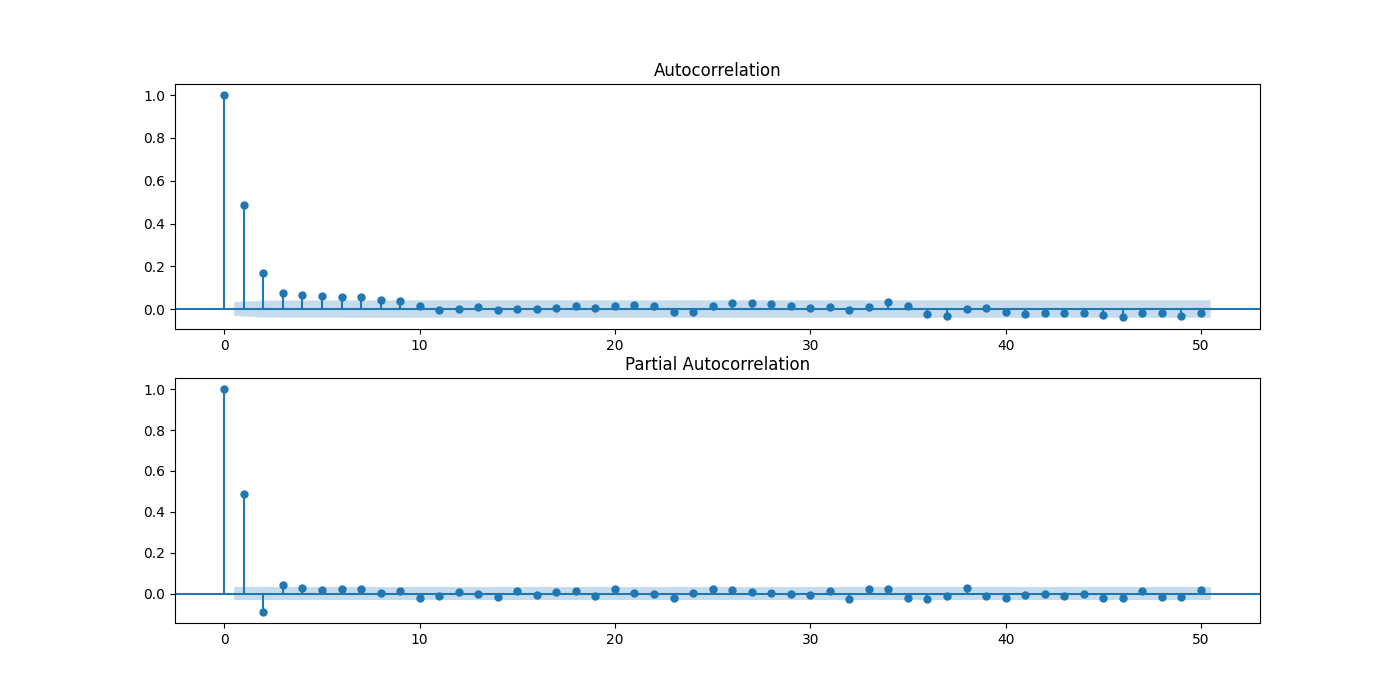
\includegraphics[width=\textwidth]{figures/Ass1/Ass1_D1_PACF_ACF.png}
    \end{minipage}
    \caption{A plot of the \gls{ACF} and \gls{PACF} of the first dataset.}
    \label{fig:Ass1_D1_PACF_ACF}
\end{figure}

\begin{figure}[H]
    \centering
    \begin{minipage}[b]{1\textwidth}
        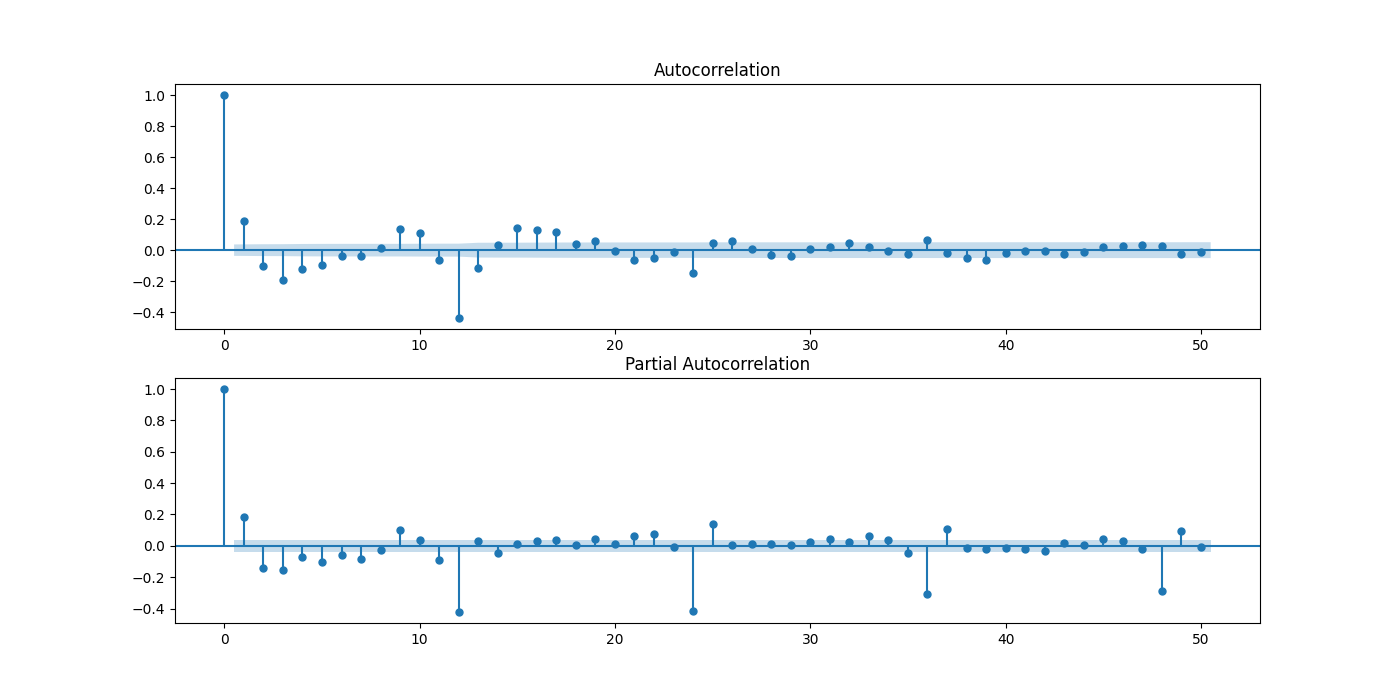
\includegraphics[width=\textwidth]{figures/Ass1/Ass1_D2_PACF_ACF.png}
    \end{minipage}
    \caption{A plot of the \gls{ACF} and \gls{PACF} of the second dataset.}
    \label{fig:Ass1_D2_PACF_ACF}
\end{figure}


\textit{These two plots are used to find the q and p for the ARIMA model. For example, if \gls{ACF} decays towards zero, and \gls{PACF} have only q significant value then our time series is a AR(q) process.}

\begin{table}[H]
\centering
\caption{The combination of the result of the \gls{KPSS} and \gls{ADF}.}
\label{tab:1}
% Please add the following required packages to your document preamble:
% \usepackage[table,xcdraw]{xcolor}
% If you use beamer only pass "xcolor=table" option, i.e. \documentclass[xcolor=table]{beamer}
\centering
\begin{tabular}{|l|l|l|}
\hline
KPSS test      & KDF test       & The combination result                      \\ \hline
non-stationary & non-stationary & The series is non-stationary.               \\ \hline
stationary     & non-stationary & Use detrending to make series stationary.   \\ \hline
non-stationary & stationary     & Use differencing to make series stationary. \\ \hline
stationary     & stationary     & The series is stationary.                   \\ \hline
\end{tabular}

\end{table}

\textit{The below figures (figure \ref{fig:Ass1_D1_Lag_Plots} and \ref{fig:Ass1_D2_Lag_Plots} ) show the lag plot of the two datasets. In each figure, there are four lag plots. As these plots illustrate, both datasets are linear, therefore our time series are a AR process.  }


\begin{figure}[H]
    \centering
    \begin{minipage}[b]{1\textwidth}
        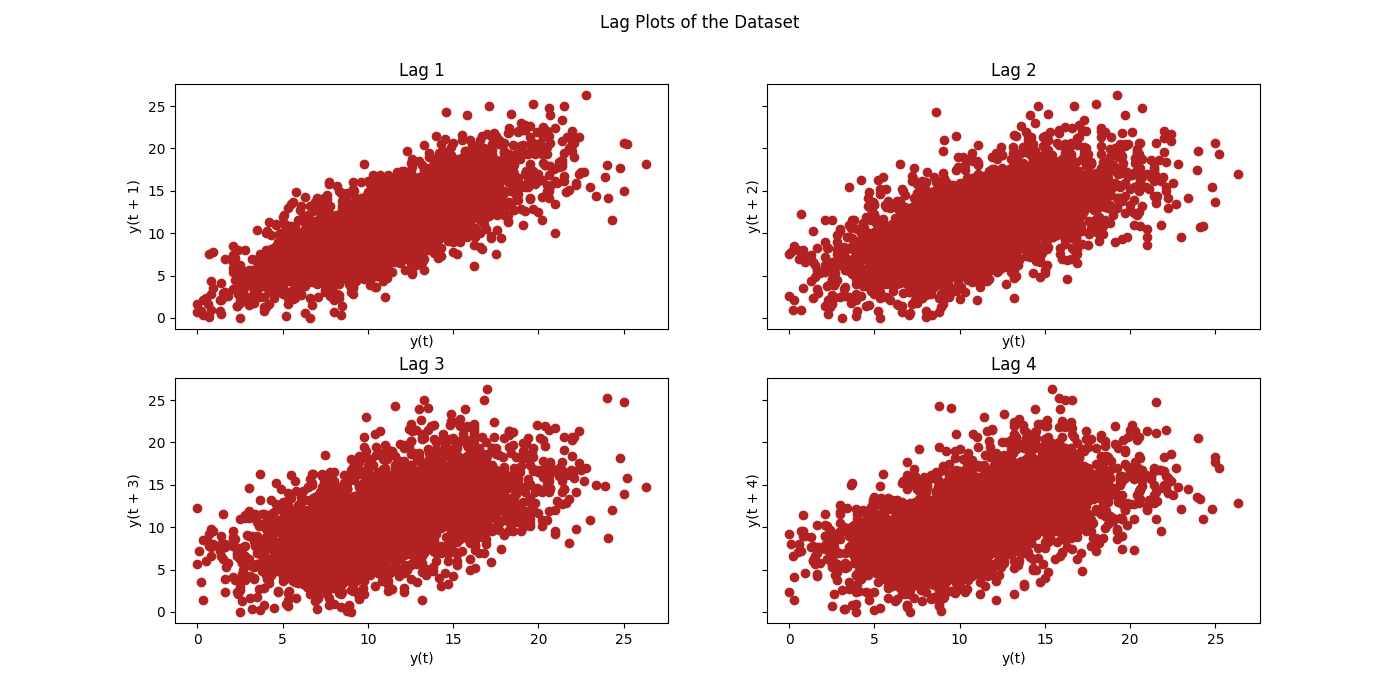
\includegraphics[width=\textwidth]{figures/Ass1/Ass1_D1_Lag_Plots.png}
    \end{minipage}
    \caption{A different lag plot of the first dataset.}
    \label{fig:Ass1_D1_Lag_Plots}
\end{figure}

\begin{figure}[H]
    \centering
    \begin{minipage}[b]{1\textwidth}
        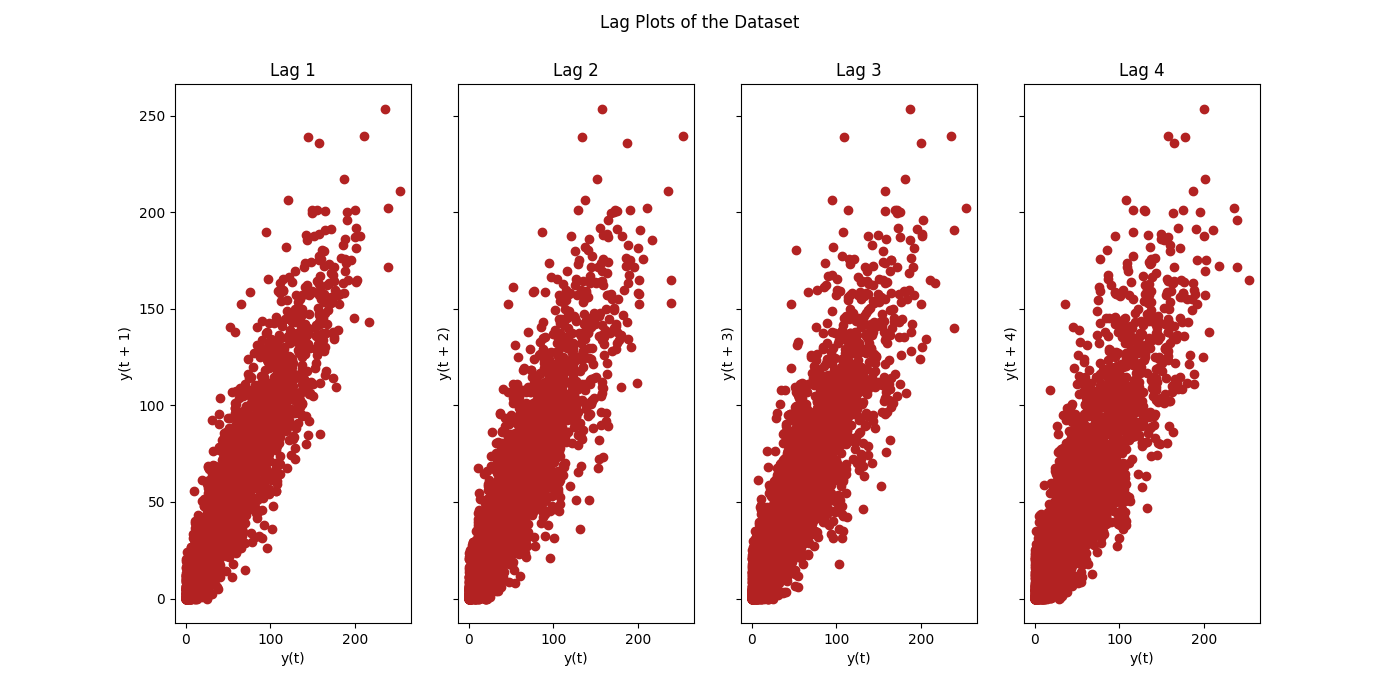
\includegraphics[width=\textwidth]{figures/Ass1/Ass1_D2_Lag_Plots.png}
    \end{minipage}
    \caption{A different lag plot of the second dataset.}
    \label{fig:Ass1_D2_Lag_Plots}
\end{figure}




\begin{figure}[H]
    \centering
    \begin{minipage}[b]{1\textwidth}
        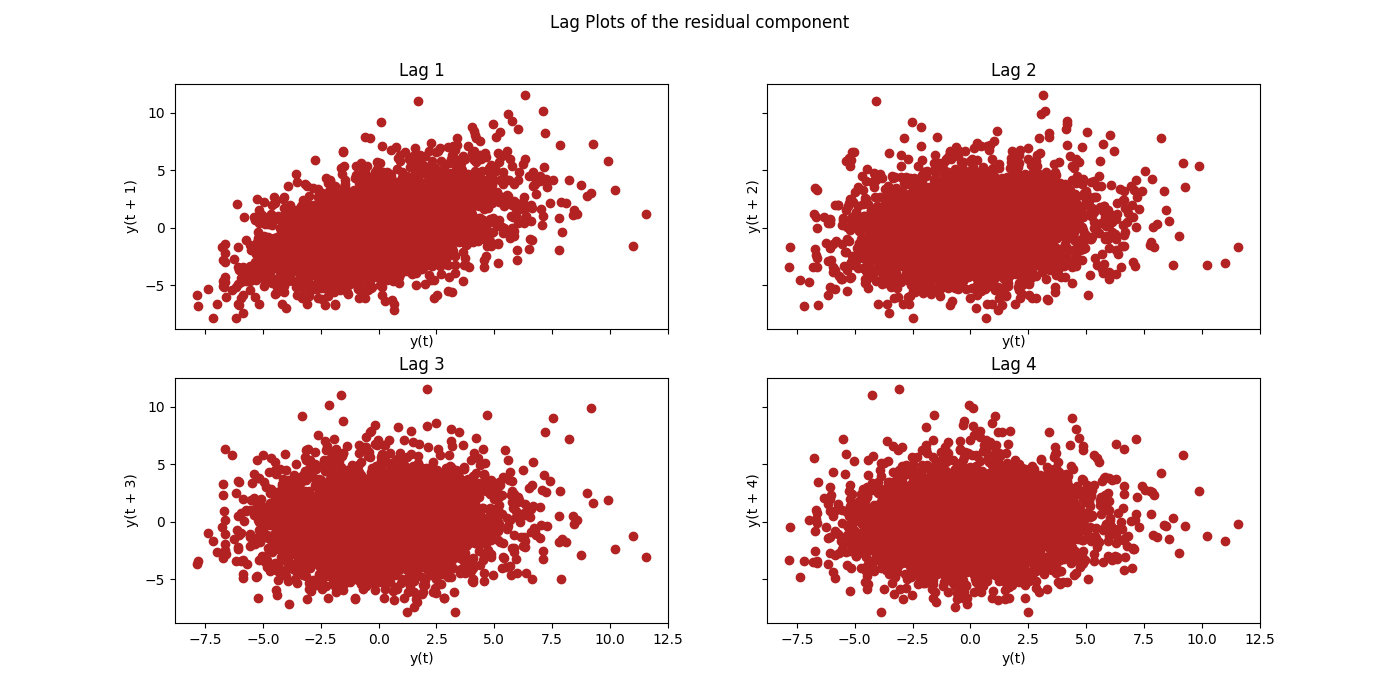
\includegraphics[width=\textwidth]{figures/Ass1/Ass1_D1_Lag_Plots_residual.png}
    \end{minipage}
    \caption{A different lag plot of residual component of the first dataset.}
    \label{fig:Ass1_D1_Lag_Plots_residual}
\end{figure}

\begin{figure}[H]
    \centering
    \begin{minipage}[b]{1\textwidth}
        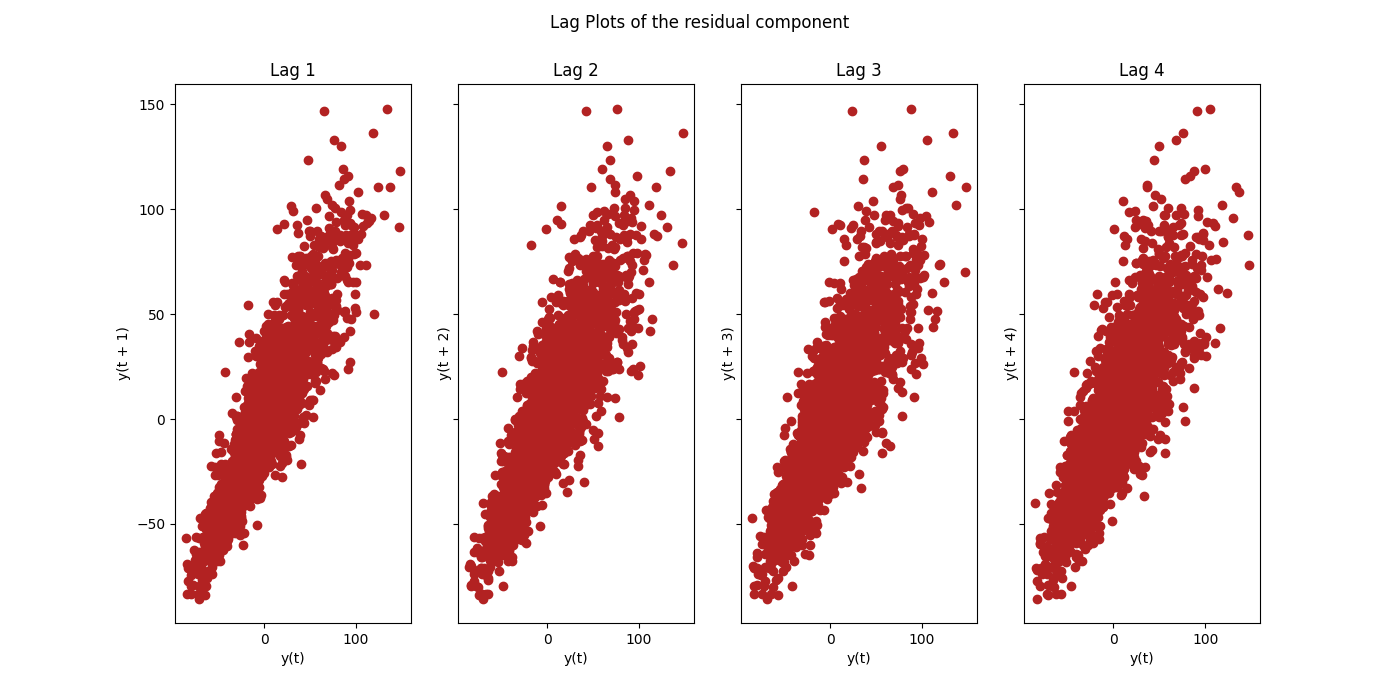
\includegraphics[width=\textwidth]{figures/Ass1/Ass1_D2_Lag_Plots_residual.png}
    \end{minipage}
    \caption{A different lag plot of residual component of the second dataset.}
    \label{fig:Ass1_D2_Lag_Plots_residual}
\end{figure}

